\documentclass[11pt,harvard]{article}
\usepackage[letterpaper, top=1in, bottom=1in, left=1in, right=1in]{geometry}
\usepackage{graphicx}
\usepackage[sort]{natbib}
\usepackage{amssymb}
\usepackage{amsmath}
\usepackage{setspace}
\usepackage{url}
\usepackage{pdflscape}
\usepackage{longtable}
\usepackage{threeparttable, booktabs}
\usepackage[export]{adjustbox}
\usepackage{enumitem}
\usepackage{comment}
\usepackage{subcaption}
\usepackage{lmodern}
\usepackage[T1]{fontenc}
\usepackage{setspace} % Load the setspace package
\usepackage{parskip} % Load the parskip package
\usepackage{float}
\usepackage{subcaption}
\usepackage{hyperref}
\usepackage[table,xcdraw]{xcolor}


\title{Sampling for the rCARI Validation Study - Iraq (IRQ)} 
\author{- rCARI Study Team - WFP, ROME - 	\\	\\For enquiries contact:\\	\\alirah.weyori@wfp.org or lena.hohfeld@wfp.org} 
\date{\today}



\begin{document}
	\maketitle \vspace{-2cm}
	\onehalfspacing
	\pagebreak
	\setlength{\parskip}{8pt} % Set the desired space before and after paragraphs
	
	% -------	
	\section{Background}
	
	The rCARI validation study is a global research project commissioned by WFP and funded by the BHA to investigate and compare remote and face-to-face (F2F) modules of the consolidated approach for reporting indicators of food insecurity (CARI). 
	The overall goal of the study is to understand to what extent food insecurity reported by rCARI is comparable or compatible with the standard CARI. Both phone (remote) and face-to-face (F2F) data collection modules \& methodologies for collecting food insecurity will used in the study.
	
	Iraq was included as part of the rCARI validation study to assess the performance of the two modalities acrossminority populations such as IDPs (Internally Displaced Persons) and Refugee populations. 
	
	Iraq has 18 Administrative regions (Governorates) with a total population of about 46 million. Though food security is not an issue amongst the general Iraqi population, food insecurity is a major issues amongst small minority groups who are mostly IDPs made up of local ethnic minorities and Syrian Refugees. The prolonged conflict in the Iraq and surrounding countries has increased the number of IDPs and Refugees in the country. For example, as at 2023, there were a total of 1.2 million IDPs in Iraq some of who face significant barriers to return to their livelihoods or be effectively integrated into the local population thereby ultimately impacting on their food security needs. In recent times, the central Government has started a policy to close all IDP and Refugee camps to reintegrate them into the general population tom increase national harmony, cohesion and development. In the process, IDP and refugee populations are facing secondary displacements fuelled by a lack of livelihood opportunities, limited services like water, sanitation, and hygiene (WASH), housing, electricity, monthly food rations, and security concerns. This situation has left these groups a more vulnerable than when they were in the camps. Aside the main validation of the remote modality, the pilot will also provide first hand food security assessment data for these minority groups within the larger population hence the reason for targeting these groups of households for the pilot study in Iraq. 
	  
	This document outlines the study methodology, specifically the sampling process adjusted for country specific context of Iraq. The study will implemented as a survey experiment with stratified sample selected across 2 regions (ADMIN1) in each pilot country.
	
	
	\section{Overall sampling design}
	
	The following considerations underpin the study areas and final sample selection.
	
	\begin{itemize}[left=2.0em]
		\item Presence of returnee IDP and or refugee households
		\item Phone ownership \& coverage within the country
		\item Areas of accessibility adjusting for difference in livelihoods
		\item Distribution of food insecurity prevalence: Representing areas with varying levels of acute food insecurity (AFI) to capture diverse food security scenarios.
	\end{itemize} 
	
	It is important to note that the primary objective of this pilot study is not to generate population-level food security estimates. Rather, the study aims to compare the effectiveness of conducting food security assessments remotely to the standard Face-to-Face (F2F) method within using the same population with comparable observable characteristics. While including diverse livelihood zones from both urban and rural communities can provide insights into modality-specific impacts, achieving national coverage and representativeness is not the focus of this study and is thus not considered in this pilot. 
	
	Iraq presents a unique context, with the study targeting IDP and refugee populations. Consequently, the sampling process has been adjusted to reflect the specific needs of these populations. The steps used to identify and select the administrative areas that will be included at various stages are outlined below.
	
	\begin{figure}[H]
		\begin{center}
			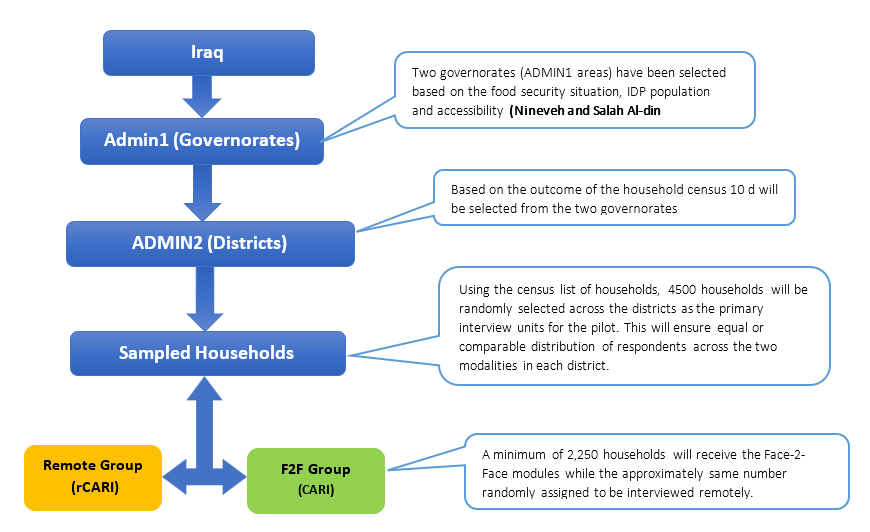
\includegraphics[scale=.75]{2_figure/IRQ_Sampling.png}
		\end{center}
		\label{fig:IRQ_Sample_Composition}
		\caption{Sample selection in Iraq}
	\end{figure}
	
	\subsection{Step 1 - Selection of ADMIN1 (Livelihood Zones)}
	The first stage involves identifying and selecting ADMIN1 (livelihood zones) that meet the inclusion criteria. In Iraq, two ADMIN1 (Governorates) areas will be purposively selected, based on recommendations from WFP country offices following the stated criteria above.
	
	Based on numbers and information received from the CO, Nineveh and Salah al-Din Governorates were the two ADMIN1s with the highest returnee IDP populations and thus have been earmarked as the pilot areas for the study.
		
	\begin{itemize}[left=2.0em]
		\item[1.] Nineveh Governorate
		\item[2.] Salah Al-din Governorate
	\end{itemize}
		These two Governorates have been selected (purposively) primarily because of the presence of IDP returnees, diversity of livelihoods, and accessibility criteria. Furthermore, these areas have been selected to capture households with varied and diverse livelihood activities as much as possible that will allow for the testing of the income source and income change indicator across different livelihoods. 
	
	\subsubsection{Nineveh Province}
	Nineveh Province is the second largest city in Iraq both in terms of population and area, after Baghdad. The province as at the end of 2023 had over 4.2 million inhabitants across 10 districts. Nineveh experienced a huge displacement and damage during the ISIS crisis with most of the inhabitants moving into IDP shelters (camps). Since 2019 due to the policy of the central government to close down these camps, almost 2 million IDPs have since returned to Nineveh out of total returnees of around 4.8 million across the country this is according to the Displacement Tracking Matrix of the IOM. These returnees are live across the 10 districts of the governorate and currently being re-integrated into the Nineveh society. 
	
	\subsubsection{Salah Al-din}
	The Salah Al-din is a central governorate in Iraq that shares borders with Kirkuk, Diyala, Al-Anbar, and Mosul. The estimated population in 2023 was 1.8 million and the majority of the residents are Sunni Arabs. The capital city, Tikrit, is significant for being Saddam Hussein's birthplace and a crucial centre of power for Sunni Arabs. Salah al-Din is home to strategically important refineries. This is also one of the governorates with a substantial number of returnee IDPs who were displaced due to the ISIS conflict in Iraq. The governorate has a total of 11 districts and the IDPs are found in all of these districts with no data on the actual numbers per district.
	
	\subsection{Step 2 - Selection of ADMIN2 (Districts) }
	In the second stage to ensure consistency in the sampling process, the same inclusion criteria as in step 1, 10 ADMIN2 areas will be purposively selected - Five from each Governorate. The number of ADMIN2s may be adjusted upwards if necessary based on the final number of districts that may meet the criteria. Furthermore, the selections will be done with special consideration given to locality, i.e., to cater for a mix of rural and urban households localities. This will ensure that livelihood activities prevalent in both rural and urban areas such as formal employment, self-employment and agricultural activities are captured as this is important for one of the key outcomes of this validation study - the income source and income change indicator.
	ADMIN2s will be regarded as the Primary Sampling Units (PSUs) in Iraq.
	
	\subsection{Step 3 - Sampling of households (HHs)}
	The final stage of the sampling procedure involves conducting a full census of all returnee households in the selected districts using the secondary data from IOM. This data includes the phone numbers of all registered returnees in the two Governorates and will therefore be used to contact and interview the households for the census exercise. During the household census, a baseline questionnaire will be administered over the phone to collect some basic observable household and respondent characteristics that will be used during the randomization phase to ensure comparability of the study groups. 
	
	In Iraq because the pilot will be amongst returnee households presents a unique challenges in identifying their precise locations. To address this, a modified approach will be used:
	\begin{itemize}
		\item Phase 1 - Census of Returnee Households:
		Using monitoring data from WFP and partner organizations such as IOM, a census of returnee households will be conducted via mobile phone calls. This census will identify households within the pilot areas and obtain their consent for inclusion in the sampling frame.
		\item Phase 2 - Baseline Data Collection:
		Demographic, socioeconomic, and physical location information (e.g., physical household address) of these households will be collected remotely using a standardized questionnaire administered by trained enumerators.
	\end{itemize}
	
	The census data which will contain the names of all household that consented to be included in the study will serve as the sampling frame for each district. Respondents for the study will then be selected following a simple random sampling approach from the sampling frame, ensuring equal selection probability for all returnee households in each of the PSUs as practicable as possible. To account for potential attrition, the study will aim to sample a minimum of 200 households per PSU (or smaller depending on the final PSUs that will be selected). A total of 4,000 returnee households will be selected for the study across the two ADMIN1 Governorates.
	
	\subsection{Step 4 - Randomization of Study Household (Sample)}
	Following the finalization of the sampling process, selected households (study sample) will be randomized into two statistically comparable groups based on their baseline observable characteristics collected during the census exercise. These two groups will then receive the F2F and remote interview modalities:
	\begin{itemize}
		\item F2F (CARI group): Households will participate in face-to-face interviews using the standard CARI methodology.
		\item Remote (rCARI group): Households will participate in phone interviews using the rCARI methodology.
	\end{itemize}

	The randomization process will ensure that the sample is equally divided between the two groups and that they two are statistically identical a pre-requisite for the comparison of the responses and data from the two modalities and groups.
			
	\begin{figure}[H]
		\begin{center}
			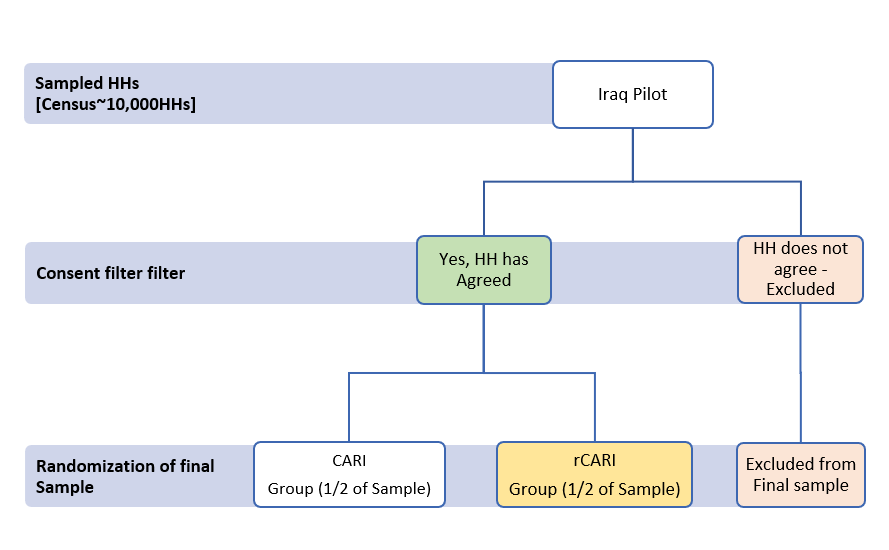
\includegraphics[scale=.70]{2_figure/IRQ_Randomization.png}
		\end{center}
		\label{fig:Sample_Randomization}
		\caption{Step by step randomization of the survey sample}
	\end{figure}
	
	\subsection {Implementation timeline}
	All interviews, both F2F and remote, will be conducted simultaneously over the same time frame. This ensures that households report on their food security status within the same reference period and are affected by similar geographical and seasonal conditions.
	
	% -------	
	\pagebreak
	% -------

	\section{Training \& assignment of enumerators}
	
	To be engaged as an enumerator for both the listing and data collection exercises, all potential enumerators should have; 
	\begin{itemize}[left=2.0em]
		\item [1.] At least a university degree,
		\item [2.] First hand knowledge of the study areas (must speak the local language/dialect), and 
		\item [3.] Prior data collection experience (at least must have been involved in two separate food security surveys) in Mauritania. 
	\end{itemize}
	
	To ensure consistency in data collection, a 4-day in person training will be organized for both F2F and remote enumerators. The enumerator training will be conducted jointly by the Iraqi CO (VAM team) and the rCARI team from HQ. Training will be largely conducted in Arabic. Local dialects will be used in cases where required to increase comprehension.
	A day's hands-on field pilot will be conducted at the end of the training session to test both the practical knowledge of enumerators and interview instruments for both modalities (F2F and remote).
	A comprehensive field guide translated into Arabic will be prepared at the end of the training and shared with enumerators to be used as quick reference in the field. In addition, field supervisors with adequate understanding of food security and livelihoods of the study area will be engaged to work closely with all enumerators in the field to increase data quality.
	
	\section{Possible limitations \& suggested mitigation strategies}
	
	Although a lot of thought has been given to the methodological design of the study, it must be mentioned that there remain some potential unavoidable sources of biases in the current experimental design setup. The potential sources and how the current design would remedy or reduce them are discussed below. 
	
	\textbf{1.} Lack of representativeness of the survey sample across the two regions. The sample may lack full representativeness across the two regions due to the inclusion of specific populations, such as IDPs or households in conflict-affected areas. This limitation is inherent in the study’s objective to include these populations and reflects the context of the regions studied. As a mitigation strategy, the household census would be broad and inclusive as much as practicable, leveraging the most recent contact information from WFP, IOM, and other partner organizations. Similarly, proportional sampling within district sampling frames to avoid over representation of certain districts will be employed so that the final sample size would not be skewed to overly represented districts in the two governorates. This will ensure the testing of the two modalities using the same sample and context as much as possible.
	
	\textbf{2.} Possible low response rates in the final sample affecting the final analysis. It is expected that the phone survey will have lower response rate than F2F, thus skewing the results more towards the F2F modality which can affect the final results. To address this limitation and ensure that the final interviewed sample is large enough to allow for statistical analysis, a number of strategies will be adopted. 
	\begin{itemize}
		\item Selective rollout of the pilot: The study will be implemented only in areas where both F2F and remote surveys are feasible.
		\item Pre-survey sensitization: During the household census, enumerators will inform respondents about the study's objective and also record preferred times for contact particularly for the remote interviews
		\item Increase the number of follow-up attempts: Specifically, in addition to the stated time by respondents to contacted, 3 additional time windows, i.e., mornings, afternoons and evenings will be used to try to contact potential respondents for the surveys. This will ensure that more households are reached within the survey period.
	\end{itemize}  
	
	\textbf{3.}	Confounding through enumerator effects (gender, training and motivation): Enumerator characteristics (e.g., gender, training quality, and motivation) may inadvertently influence the survey results, especially since the same enumerator cannot conduct both F2F and remote interviews simultaneously. Knowing this, the study will adopt the following mitigation strategies to minimise or at best eliminate these inherent biases.
	\begin{itemize}
		\item Random Assignment: Enumerators will be randomly assigned to districts and modalities, ensuring at least two enumerators per district with balanced gender representation.
		\item Unified Training: All enumerators will receive the same training from a single team of facilitators, followed by a knowledge test to assess comprehension of the questionnaire by enumerators and or the retraining or replacement of low-performing enumerators based on test results.
		\item Performance monitoring during data collection exercise: A dedicated data quality team will be conducting daily high-frequency checks to evaluate enumerator performance. Enumerators found to consistently record questionable data will either be asked to re-conduct interviews or replaced if issues persist after caution.
		\item Increase female enumerator representation: More female enumerators will be assigned to remote interviews, as evidence suggests they achieve higher response rates in phone surveys. Similarly, as much as possible, more females will also be recruited to be deployed for the F2F as well.
	\end{itemize}
	
\end{document}